\chapter{Phase III}

\section{Structur of software}
The figure \ref{fig:phase3} shows the implementation details behin the \emph{Opponent Model Strategy}. The \emph{Opponent Logger} tracks all the actions that are made by all players and associates them with the context at which these actions have been made. These actions are stored as list of \emph{Opponent Entry}-objects. 

At the show down all the players that are still in the game have to show their cards. Now the \emph{Opponent Entry}-list of these players is went through. The player's cards are combined with the share cards and the hand strength is computed. The hand strength is committed to the \emph{Opponent Model} together with the current context and the player's action.

\begin{figure}[h]
  \centering
  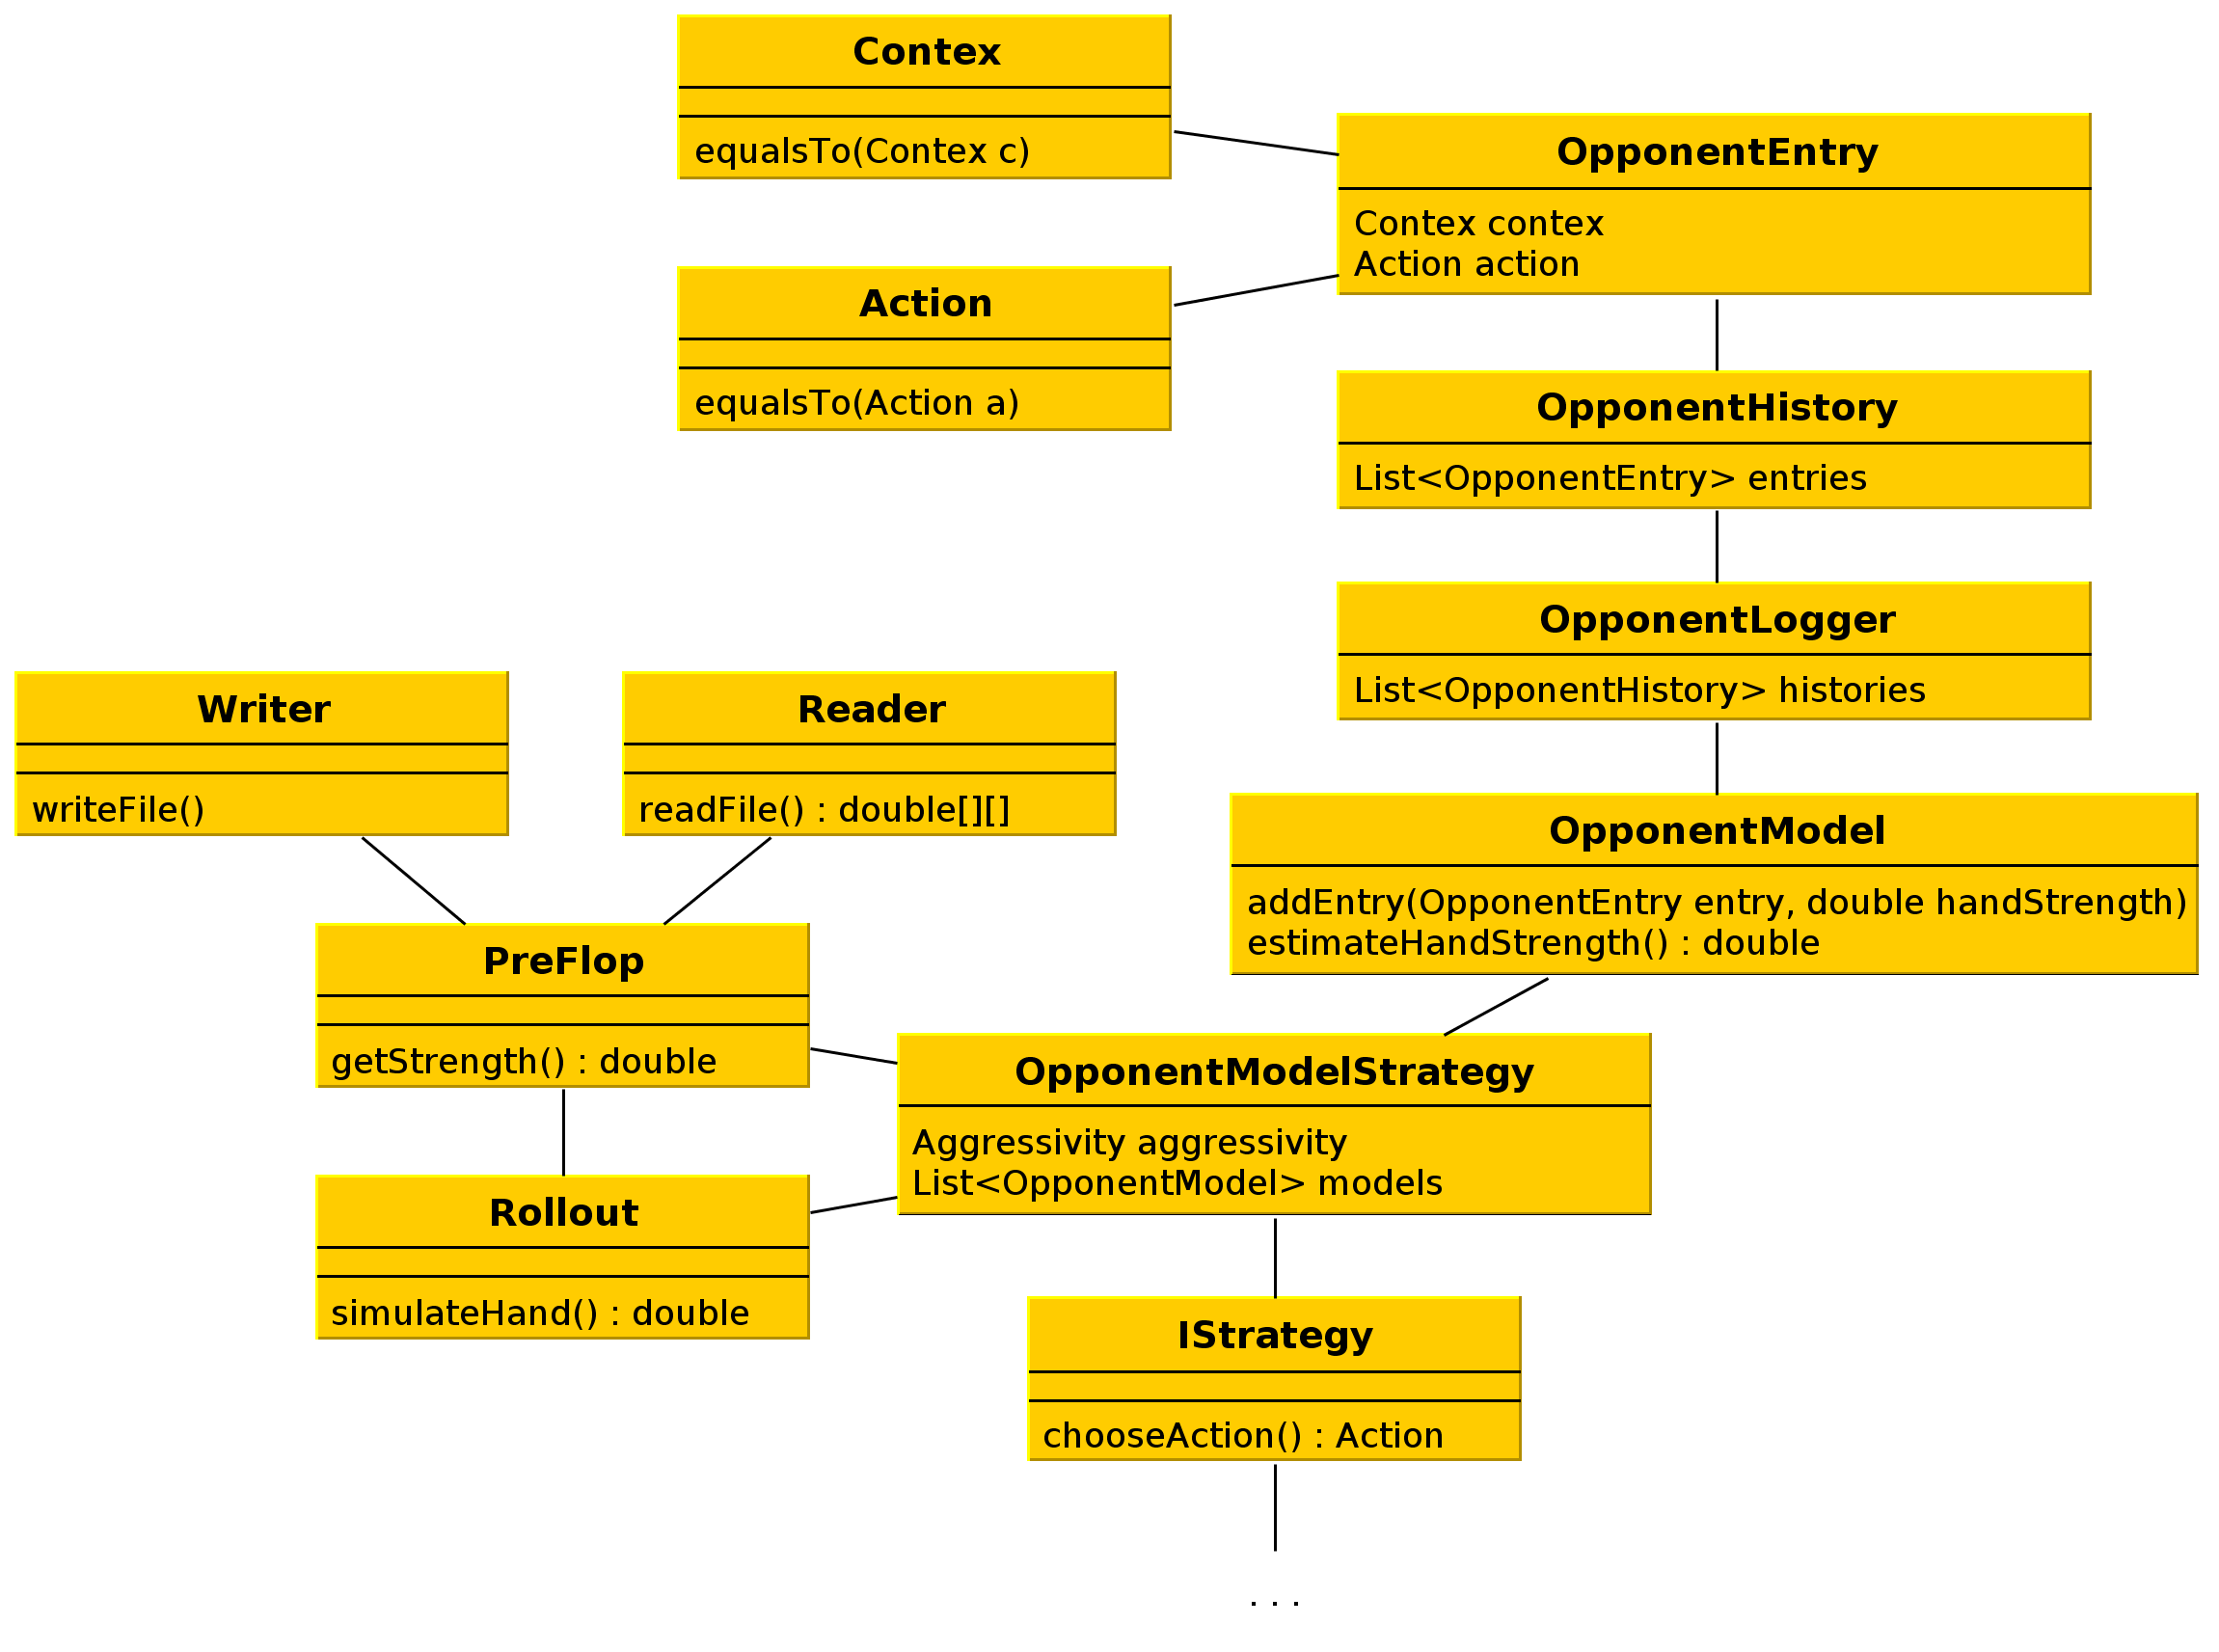
\includegraphics[width=1.0\textwidth]{images/phase3}
  \caption{Software design of phase III}
  \label{fig:phase3}
\end{figure}

\section{Opponent model}
Basically the phase III player acts the same way like phase II player does. The only difference is, t

\section{Results}

